\documentclass[10pt]{article}
\usepackage[top=1in,bottom=1.1in,left=.8in,right=.8in]{geometry}
\usepackage[T1]{fontenc}
\usepackage[ansinew]{inputenc}
\usepackage{graphicx}
\usepackage{multirow}
\usepackage{enumitem}


\renewcommand{\familydefault}{\sfdefault}

\begin{document}
%\maketitle

\hspace{-5mm}
\begin{minipage}{0.65\linewidth}
  \textbf{
      \hspace{-3mm}
      {\Large COMP 231-01}\\
      {\Large Introduction to Computer Organization}\\
      {\Large Exam Review}}
\end{minipage}
\begin{minipage}{0.35\linewidth}
  \includegraphics[scale=.3]{../../logos/rhodes-logo.jpg}
\end{minipage}

%\noindent{\bf Due Date: Monday, February 13th.}\\
%\noindent{\bf Due Date: Monday, September 19th.}\\
%\noindent{\bf Due Date: Tuesday, September 26th.}\\
%\noindent{\bf Due Date: Thursday, September 27th.}\\
%\noindent{\bf Due Date: Friday, February 8th.}\\
%\noindent{\bf Due Date: Monday, September 16th.}\\



\begin{itemize}

\setlength\itemsep{10mm}


\item Answer the following questions:



  \begin{enumerate}
\setlength\itemsep{5mm}
\item Convert the following to base-10:
\begin{enumerate}[label=\Alph*]

\item $21_3$   \textbf{7}

\item $371_{17}$ \textbf{987}

\item $100111_2$ \textbf{39}

\item $52_6$ \textbf{32}

\item $FB_{16}$ \textbf{251}

\item $71_9$ \textbf{64}

\item $1B1_{16}$ \textbf{433}

\item $11_2$ \textbf{3}

\end{enumerate}

\item Convert the following from decimal notation to the corresponding base:
\begin{enumerate}[label=\Alph*]


\item $533$ to base 2   \textbf{1000010101}

\item $2062$ to base 2   \textbf{100000001110}

\item $12$ to base 2   \textbf{1100}

\item $243$ to base 16  \textbf{F3}

\item $27$ to base 16   \textbf{1B}

\item $5000$ to base 16   \textbf{1388}

\item $11$ to base 5   \textbf{21}

\item $66$ to base 3  \textbf{2110}
\end{enumerate}

\item Convert the following from decimal to 8-bit 2's complement:
\begin{enumerate}[label=\Alph*]


\item $-100$   \textbf{11100100}

\item $32$   \textbf{00100000}

\item $-57$  \textbf{11000111}

\item $67$   \textbf{01000011}

\item $-128$  \textbf{10000000}

\item $128$  \textbf{Undefined!  Out of bounds for 8-bit 2's complement}

\end{enumerate}

\item Perform the following operations using 4-bit 2's complement signed arithmetic:
\begin{enumerate}[label=\Alph*]


\item $0110 + 1001$    \textbf{1111}

\item $1010 + 0011$    \textbf{1101}

\item $1110 + 0101$    \textbf{0011  carry out = 1}

\item $1100 + 0111$   \textbf{0011  carry out = 1}

\item $1011 - 1001$   \textbf{1011 + 0111 = 0010 carry out = 1}

\item $0011 - 0010$   \textbf{0011 + 1110 = 0001 carry out = 1}

\item $1001 - 0011$  \textbf{1001 + 1101 = 0110 carry out = 1}

\item $0001 - 0110$  \textbf{0001 + 1111 = 0000 carry out = 1}


\end{enumerate}

\item Consider the boolean algebra expression $F = \bar{A} *B + A*B*C$.  Create a k-map for this expression and use the k-map to derive the MSOP (minimal sum of products).

\item Consider the boolean algebra expression $F = \bar{A}\bar{B}\bar{C}\bar{D}+\bar{A}\bar{B}C\bar{D}+\bar{A}BC\bar{D}+\bar{A}BCD+A\bar{B}\bar{C}\bar{D}+ABC\bar{D}+ABCD$.  Create a k-map for this expression and use the k-map to derive the MSOP (minimal sum of products).

\item Create a truth table, a MSOP boolean algebra expression, and draw a circuit for a function that takes in two variables and returns 1 if the function is even and 0 if the function is odd.  (For this situation, we don't care whether a zero is evaluated as even or odd.) \textbf{For this problem, use only and gates, or gates, and not gates.}

\item Create a truth table, a MSOP boolean algebra expression, and draw a circuit for a function that takes in three variables and returns 1 only if two of the inputs are 1. \textbf{For this problem, use only and gates, or gates, and not gates.}

\item Consider the following circuit, with a T flipflop and a JK flip flop.  Create a characteristic table that shows what the next state will be for this circuit. 

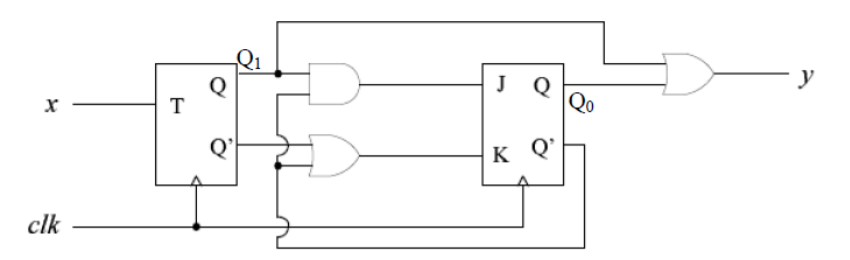
\includegraphics[scale=.8]{ExampleFFProblem.png}

\item Consider the following circuit.  What is the characteristic table for its output?

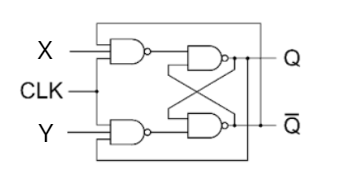
\includegraphics[scale=.8]{FlipFlopBehaviourProblemWithLabels.png}

\item What is the use of a half adder?  In what situation would this be used?

The half adder adds two inputs together.  This would be used if you're adding the first digit of a number.

\item What is the characteristic table for the D flipflop?

D = 0, Q = 0

D = 1, Q = 1

\item Why is state S=1 R=1 undefined for an SR flipflop?

Because the transition to S=0 R=0 results in a race condition and undefined behavior.  Also because it violates our rule that Q and $\bar{Q}$ are opposites.

\item Is this 64-bit signed 2's complement number positive or negative? \\
1000011000101110111101001111100011101001111001100001101101010101

Negative, from the first bit.

\item What is the purpose of a multiplexer?

It toggles between different data streams based on a set of switches, allowing each data input access to the circuit or device.

\item What is the range of 8-bit signed 2's complement?

-128 to +127

\item What is the difference between 1's complement and 2's complement?

In 2's complement, you add 1 to the result of 1's complement

\item What is a decoder used for in an ALU?

It is used to select which operation is run.

\item How do we implement memory in our circuits?

We use flip flops to incorporate the idea of memory (feedback).  They can be used to store values even from previous clock cycles.

\item What is the disadvantage of a ripple-carry adder?

A ripple carry-adder needs time for all the bits to calculate their carry out, each of which depends on the previous bit.  This can produce incorrect results if the value is read before the carry out values have propogated all the way through.

\end{enumerate}

\end{itemize}

\end{document}

